\documentclass{article}

\usepackage{enumerate}
\usepackage{graphicx}

\title{Homework 1}
\author{Connor Taffe}

\begin{document}
	\maketitle

	The following outlines a report of Artificial Intelligence's Homework One. I include both the {\tt main.c} solution (Compiles with {\tt make} on {\it Linux}, {\it BSD}, and {\it OS X}. Very impressive 0.161s execution time for 1000 restarts on my machine. Optional Runge-Kutta classic simulation and PCG random numbers.), and the hastily programmed {\tt C++} version which compiles on {\it Windows}.

	I encourage you to run the {\tt C++} version, but investigate the {\tt C} version for more aesthetically appealing code and functional identicity.

	\section{Compiling the code}

	\begin{enumerate}
		\item{Open {\tt main.cc} in Visual Studio.}
		\item{Hit {\tt F5}.}
	\end{enumerate}

	\section{Running the code}
		\begin{enumerate}
			\item{Hit {\tt F5} again?}
		\end{enumerate}

	\section{Plot}

	The following is the scatter plot with the cost ($y$) as a function of the number of evals ($x$), $y = f(x)$. Seen in figure \ref{plot}.

	\begin{figure}[h]
		\centering
		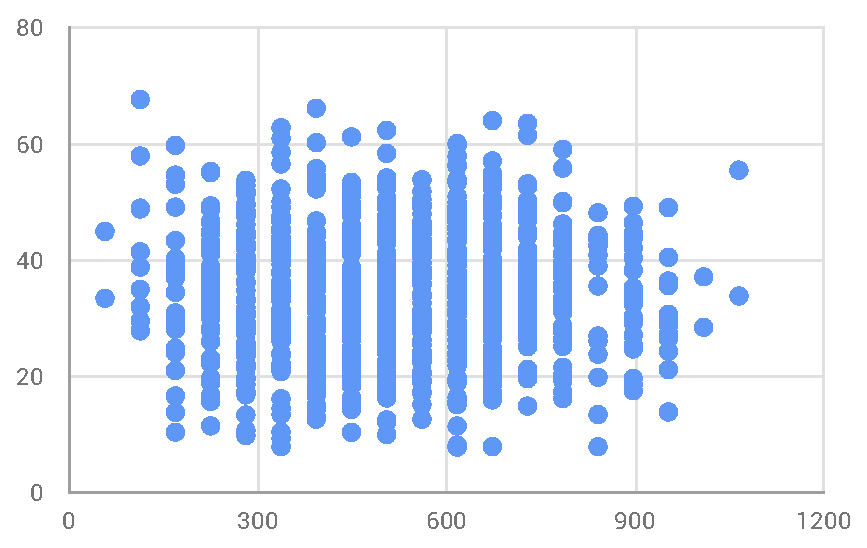
\includegraphics[width=250pt]{plot}
		\caption{\label{plot} Scatter Plot}
	\end{figure}

	\section{Report}

	Here follows the report sections as outlined in the spec.

	\begin{enumerate}[(a)]
		\item{
			The local search implements {\it Greedy-Descent} ({\it Steepest-Descent}), so it pursues the lowest error neighbors ($O(n)$ testing) towards a local mimuma. Shoulders would end the search as would plateus. Any rise in the error landscape would terminate the search. They only redeeming quality of the program is that since it randomly sampled so much, many times landing on local mimima slopes, the landscape was somewhat navigated (applies to all local search).
		}
		\item{
			With 1000 random restarts and an average neighbor-follow length of around 9 hamming distances, I would assume the local search had a fairly good navigation of even such a large space.
		}
		\item{
			An intermediate solution is a solution that is not a terminating local maxima. These are solutions that have one hamming distance nieghbors with a lower cost. They are on a slope of the error landscape.
		}
		\item{
			The error function defines the error landscape, or how the local search moves throughout the set of possible solutions.
		}
		\item{
			Possibly, if it provided a more easily followable slope for local search. For example, an error function which creates many local minimas but one large global minima which are unassociated (rigid, sharply pitted, one deep pit) compared to one which has few far reaching slopes leading to local minima, one of which being global (smoother, bowl-like). The second is much better for local search, giving it a much larger error landscape surface to land on which leads to the global maxima.
		}
	\end{enumerate}

	\section{Suggestions}

	The ``Programming Language Policy'' section of the syllabus outlines which ``base languages'' are approved for use in this course. {\tt C} is listed as an acceptable language, which (to me) suggests that a recent standard version of {\tt C} would be appropriate for use.

	As the required environment (Visual Studio on Windows) does not actually have a {\tt C} compiler avaliable, it is fairly impossible to use a {\tt C} language program as a submission. To be fair, the {\tt C++} compiler avaliable will compile the {\tt C} standard version from 1989, but I know of nothing except {\tt git} that is programmed in {\tt C} '89. Therefore, perhaps the accepted language specification should include this information.

\end{document}
